\subsection{Plugin Architecture} \label{subsec_plugin_architecture}

When all preconditions are met and the expander is compiled, the expander consists of a
\gls{dll} and a set of templates. The Generator artifact considers the expanders as
optional plugins, which are dynamically loaded at runtime, through a method called
assembly-binding. See section \fullref{subsec_expanders} for a full explanation of the
required preconditions.

\begin{figure}[H]
  \centering
  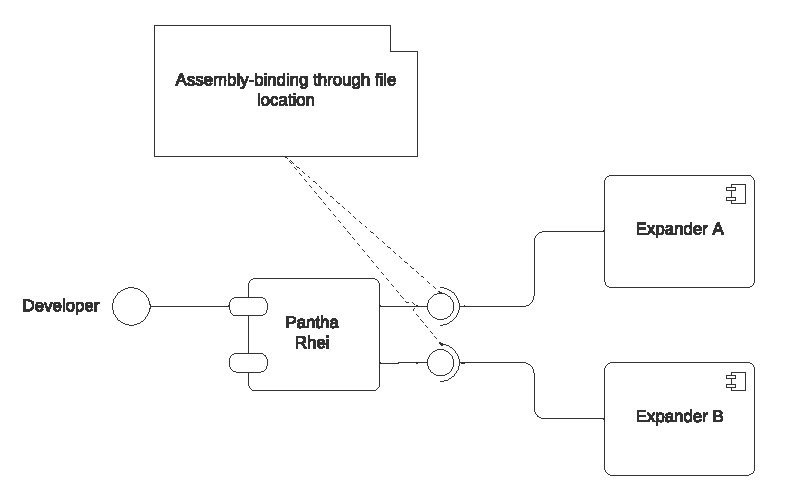
\includegraphics[width=1\textwidth]{figures/plugin_architecture.pdf}
  \caption[Plugin Archticture]{Expanders are considered plugins}
  \label{fi:plugin_architecture}
\end{figure}

By implementing the expanders as plugins, the design adheres to several \gls{solid}
principles. First and foremost, \gls{srp} is respected because an expander should generate
one, and precisely one construct \parencite[403]{mannaert_normalized_2016}. In the case of
this research, this construct is an application following the design and principles of the
design approach of \gls{ca} with a Restful API interface. Furthermore, it supports the
\gls{ocp} principles because developers can introduce a new version of the expander as a
separate plugin if this is required. \gls{lsp}. By extension, this also adheres to the
\gls{lsp} principle, as expanders can be replaced with other implementations of expanders,
without affecting the rest of the application.